% Options for packages loaded elsewhere
\PassOptionsToPackage{unicode}{hyperref}
\PassOptionsToPackage{hyphens}{url}
%
\documentclass[
]{article}
\title{Problem Set}
\author{Alberto José Díaz Cuenca and Ignacio Almodóvar Cárdenas}
\date{21/3/2022}

\usepackage{amsmath,amssymb}
\usepackage{lmodern}
\usepackage{iftex}
\ifPDFTeX
  \usepackage[T1]{fontenc}
  \usepackage[utf8]{inputenc}
  \usepackage{textcomp} % provide euro and other symbols
\else % if luatex or xetex
  \usepackage{unicode-math}
  \defaultfontfeatures{Scale=MatchLowercase}
  \defaultfontfeatures[\rmfamily]{Ligatures=TeX,Scale=1}
\fi
% Use upquote if available, for straight quotes in verbatim environments
\IfFileExists{upquote.sty}{\usepackage{upquote}}{}
\IfFileExists{microtype.sty}{% use microtype if available
  \usepackage[]{microtype}
  \UseMicrotypeSet[protrusion]{basicmath} % disable protrusion for tt fonts
}{}
\makeatletter
\@ifundefined{KOMAClassName}{% if non-KOMA class
  \IfFileExists{parskip.sty}{%
    \usepackage{parskip}
  }{% else
    \setlength{\parindent}{0pt}
    \setlength{\parskip}{6pt plus 2pt minus 1pt}}
}{% if KOMA class
  \KOMAoptions{parskip=half}}
\makeatother
\usepackage{xcolor}
\IfFileExists{xurl.sty}{\usepackage{xurl}}{} % add URL line breaks if available
\IfFileExists{bookmark.sty}{\usepackage{bookmark}}{\usepackage{hyperref}}
\hypersetup{
  pdftitle={Problem Set},
  pdfauthor={Alberto José Díaz Cuenca and Ignacio Almodóvar Cárdenas},
  hidelinks,
  pdfcreator={LaTeX via pandoc}}
\urlstyle{same} % disable monospaced font for URLs
\usepackage[margin=1in]{geometry}
\usepackage{color}
\usepackage{fancyvrb}
\newcommand{\VerbBar}{|}
\newcommand{\VERB}{\Verb[commandchars=\\\{\}]}
\DefineVerbatimEnvironment{Highlighting}{Verbatim}{commandchars=\\\{\}}
% Add ',fontsize=\small' for more characters per line
\usepackage{framed}
\definecolor{shadecolor}{RGB}{248,248,248}
\newenvironment{Shaded}{\begin{snugshade}}{\end{snugshade}}
\newcommand{\AlertTok}[1]{\textcolor[rgb]{0.94,0.16,0.16}{#1}}
\newcommand{\AnnotationTok}[1]{\textcolor[rgb]{0.56,0.35,0.01}{\textbf{\textit{#1}}}}
\newcommand{\AttributeTok}[1]{\textcolor[rgb]{0.77,0.63,0.00}{#1}}
\newcommand{\BaseNTok}[1]{\textcolor[rgb]{0.00,0.00,0.81}{#1}}
\newcommand{\BuiltInTok}[1]{#1}
\newcommand{\CharTok}[1]{\textcolor[rgb]{0.31,0.60,0.02}{#1}}
\newcommand{\CommentTok}[1]{\textcolor[rgb]{0.56,0.35,0.01}{\textit{#1}}}
\newcommand{\CommentVarTok}[1]{\textcolor[rgb]{0.56,0.35,0.01}{\textbf{\textit{#1}}}}
\newcommand{\ConstantTok}[1]{\textcolor[rgb]{0.00,0.00,0.00}{#1}}
\newcommand{\ControlFlowTok}[1]{\textcolor[rgb]{0.13,0.29,0.53}{\textbf{#1}}}
\newcommand{\DataTypeTok}[1]{\textcolor[rgb]{0.13,0.29,0.53}{#1}}
\newcommand{\DecValTok}[1]{\textcolor[rgb]{0.00,0.00,0.81}{#1}}
\newcommand{\DocumentationTok}[1]{\textcolor[rgb]{0.56,0.35,0.01}{\textbf{\textit{#1}}}}
\newcommand{\ErrorTok}[1]{\textcolor[rgb]{0.64,0.00,0.00}{\textbf{#1}}}
\newcommand{\ExtensionTok}[1]{#1}
\newcommand{\FloatTok}[1]{\textcolor[rgb]{0.00,0.00,0.81}{#1}}
\newcommand{\FunctionTok}[1]{\textcolor[rgb]{0.00,0.00,0.00}{#1}}
\newcommand{\ImportTok}[1]{#1}
\newcommand{\InformationTok}[1]{\textcolor[rgb]{0.56,0.35,0.01}{\textbf{\textit{#1}}}}
\newcommand{\KeywordTok}[1]{\textcolor[rgb]{0.13,0.29,0.53}{\textbf{#1}}}
\newcommand{\NormalTok}[1]{#1}
\newcommand{\OperatorTok}[1]{\textcolor[rgb]{0.81,0.36,0.00}{\textbf{#1}}}
\newcommand{\OtherTok}[1]{\textcolor[rgb]{0.56,0.35,0.01}{#1}}
\newcommand{\PreprocessorTok}[1]{\textcolor[rgb]{0.56,0.35,0.01}{\textit{#1}}}
\newcommand{\RegionMarkerTok}[1]{#1}
\newcommand{\SpecialCharTok}[1]{\textcolor[rgb]{0.00,0.00,0.00}{#1}}
\newcommand{\SpecialStringTok}[1]{\textcolor[rgb]{0.31,0.60,0.02}{#1}}
\newcommand{\StringTok}[1]{\textcolor[rgb]{0.31,0.60,0.02}{#1}}
\newcommand{\VariableTok}[1]{\textcolor[rgb]{0.00,0.00,0.00}{#1}}
\newcommand{\VerbatimStringTok}[1]{\textcolor[rgb]{0.31,0.60,0.02}{#1}}
\newcommand{\WarningTok}[1]{\textcolor[rgb]{0.56,0.35,0.01}{\textbf{\textit{#1}}}}
\usepackage{graphicx}
\makeatletter
\def\maxwidth{\ifdim\Gin@nat@width>\linewidth\linewidth\else\Gin@nat@width\fi}
\def\maxheight{\ifdim\Gin@nat@height>\textheight\textheight\else\Gin@nat@height\fi}
\makeatother
% Scale images if necessary, so that they will not overflow the page
% margins by default, and it is still possible to overwrite the defaults
% using explicit options in \includegraphics[width, height, ...]{}
\setkeys{Gin}{width=\maxwidth,height=\maxheight,keepaspectratio}
% Set default figure placement to htbp
\makeatletter
\def\fps@figure{htbp}
\makeatother
\setlength{\emergencystretch}{3em} % prevent overfull lines
\providecommand{\tightlist}{%
  \setlength{\itemsep}{0pt}\setlength{\parskip}{0pt}}
\setcounter{secnumdepth}{-\maxdimen} % remove section numbering
\ifLuaTeX
  \usepackage{selnolig}  % disable illegal ligatures
\fi

\begin{document}
\maketitle

\hypertarget{exercise-5.11.}{%
\subsection{Exercise 5.11.}\label{exercise-5.11.}}

The challenger.txt dataset contains information regarding the state of
the solid rocket boosters after launch for 23 shuttle flights prior the
Challenger launch. Each row has, among others, the variables fail.field
(indicator of whether there was an incident with the O-rings),
nfail.field (number of incidents with the O-rings), and temp
(temperature in the day of launch, measured in Celsius degrees).

First of all, we start by reading the dataset ``challenger.txt''. We
have stored the response variable fail.field in a variable called ``Y''
and the predictor variable temp in ``X''.

We are going to employ locfit in order to fit the logistic regression
models. Here, the bandwidth needs to be specified within the ``lp''
argument.

We started with the lowest bandwidth allowed by the model, which is
equal to h=0.22. That can allow us to believe that it will undersmooth
the function. To find a somehow adequate bandwith, we have used h=0.6,
which creates an estimation that seems correct. Finally, we have used a
bandwith h=2, which assures us an oversmoothing.

\begin{Shaded}
\begin{Highlighting}[]
\NormalTok{h}\OtherTok{=}\FloatTok{0.22}
\NormalTok{fit\_locfit }\OtherTok{\textless{}{-}}\NormalTok{ locfit}\SpecialCharTok{::}\FunctionTok{locfit}\NormalTok{(Y }\SpecialCharTok{\textasciitilde{}}\NormalTok{ locfit}\SpecialCharTok{::}\FunctionTok{lp}\NormalTok{(X, }\AttributeTok{deg =} \DecValTok{1}\NormalTok{, }\AttributeTok{nn =}\NormalTok{ h),}
                             \AttributeTok{family =} \StringTok{"binomial"}\NormalTok{, }\AttributeTok{kern =} \StringTok{"gauss"}\NormalTok{)}
\NormalTok{h2 }\OtherTok{=} \FloatTok{1.5}
\NormalTok{fit\_locfit2 }\OtherTok{\textless{}{-}}\NormalTok{locfit}\SpecialCharTok{::}\FunctionTok{locfit}\NormalTok{(Y }\SpecialCharTok{\textasciitilde{}}\NormalTok{ locfit}\SpecialCharTok{::}\FunctionTok{lp}\NormalTok{(X, }\AttributeTok{deg =} \DecValTok{1}\NormalTok{, }\AttributeTok{nn =}\NormalTok{ h2),}
                               \AttributeTok{family =} \StringTok{"binomial"}\NormalTok{, }\AttributeTok{kern =} \StringTok{"gauss"}\NormalTok{)}

\NormalTok{h3 }\OtherTok{=} \DecValTok{10}
\NormalTok{fit\_locfit3 }\OtherTok{\textless{}{-}}\NormalTok{locfit}\SpecialCharTok{::}\FunctionTok{locfit}\NormalTok{(Y }\SpecialCharTok{\textasciitilde{}}\NormalTok{ locfit}\SpecialCharTok{::}\FunctionTok{lp}\NormalTok{(X, }\AttributeTok{deg =} \DecValTok{1}\NormalTok{, }\AttributeTok{nn =}\NormalTok{ h3),}
                               \AttributeTok{family =} \StringTok{"binomial"}\NormalTok{, }\AttributeTok{kern =} \StringTok{"gauss"}\NormalTok{)}
\end{Highlighting}
\end{Shaded}

Plotting the results.

\begin{Shaded}
\begin{Highlighting}[]
\FunctionTok{plot}\NormalTok{(fit\_locfit, }\AttributeTok{col=}\DecValTok{1}\NormalTok{) }\SpecialCharTok{+} \FunctionTok{lines}\NormalTok{(fit\_locfit2, }\AttributeTok{col=}\DecValTok{2}\NormalTok{)  }\SpecialCharTok{+} \FunctionTok{lines}\NormalTok{(fit\_locfit3, }\AttributeTok{col=}\DecValTok{3}\NormalTok{) }\SpecialCharTok{+} \FunctionTok{points}\NormalTok{(X,Y, }\AttributeTok{type=}\StringTok{"p"}\NormalTok{)}
\end{Highlighting}
\end{Shaded}

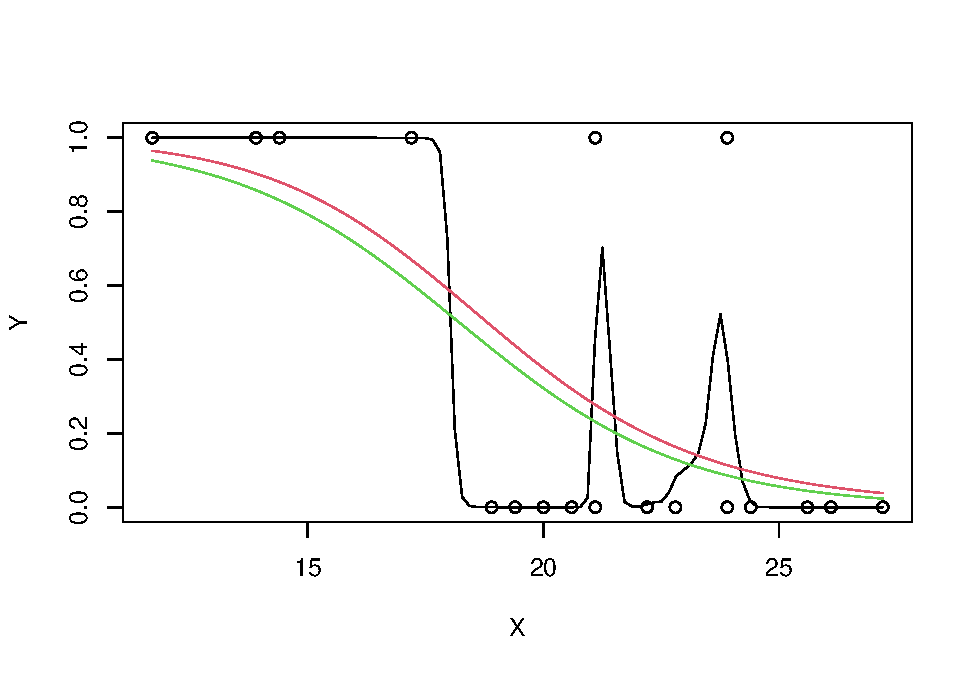
\includegraphics{Problemsetrmd_files/figure-latex/unnamed-chunk-3-1.pdf}

\begin{verbatim}
## integer(0)
\end{verbatim}

\begin{Shaded}
\begin{Highlighting}[]
\CommentTok{\# Exact LCV}
\NormalTok{h }\OtherTok{\textless{}{-}} \FunctionTok{seq}\NormalTok{(}\FloatTok{0.5}\NormalTok{, }\DecValTok{5}\NormalTok{, }\AttributeTok{by =} \FloatTok{0.1}\NormalTok{)}
\NormalTok{n}\OtherTok{=}\DecValTok{23}
\FunctionTok{suppressWarnings}\NormalTok{(}
\NormalTok{  LCV }\OtherTok{\textless{}{-}} \FunctionTok{sapply}\NormalTok{(h, }\ControlFlowTok{function}\NormalTok{(h) \{}
  \FunctionTok{sum}\NormalTok{(}\FunctionTok{sapply}\NormalTok{(}\DecValTok{1}\SpecialCharTok{:}\NormalTok{n, }\ControlFlowTok{function}\NormalTok{(i) \{}
\NormalTok{    K }\OtherTok{\textless{}{-}} \FunctionTok{dnorm}\NormalTok{(}\AttributeTok{x =}\NormalTok{ X[i], }\AttributeTok{mean =}\NormalTok{ X[}\SpecialCharTok{{-}}\NormalTok{i], }\AttributeTok{sd =}\NormalTok{ h)}
    \FunctionTok{nlm}\NormalTok{(}\AttributeTok{f =} \ControlFlowTok{function}\NormalTok{(beta) \{}
      \SpecialCharTok{{-}}\FunctionTok{sum}\NormalTok{(K }\SpecialCharTok{*}\NormalTok{ (Y[}\SpecialCharTok{{-}}\NormalTok{i] }\SpecialCharTok{*}\NormalTok{ (beta[}\DecValTok{1}\NormalTok{] }\SpecialCharTok{+}\NormalTok{ beta[}\DecValTok{2}\NormalTok{] }\SpecialCharTok{*}\NormalTok{ (X[}\SpecialCharTok{{-}}\NormalTok{i] }\SpecialCharTok{{-}}\NormalTok{ X[i])) }\SpecialCharTok{{-}}
                  \FunctionTok{log}\NormalTok{(}\DecValTok{1} \SpecialCharTok{+} \FunctionTok{exp}\NormalTok{(beta[}\DecValTok{1}\NormalTok{] }\SpecialCharTok{+}\NormalTok{ beta[}\DecValTok{2}\NormalTok{] }\SpecialCharTok{*}\NormalTok{ (X[}\SpecialCharTok{{-}}\NormalTok{i] }\SpecialCharTok{{-}}\NormalTok{ X[i])))))}
\NormalTok{      \}, }\AttributeTok{p =} \FunctionTok{c}\NormalTok{(}\DecValTok{0}\NormalTok{,}\DecValTok{0}\NormalTok{))}\SpecialCharTok{$}\NormalTok{minimum}
\NormalTok{    \}))}
\NormalTok{  \})}
\NormalTok{)}
\FunctionTok{plot}\NormalTok{(h, LCV, }\AttributeTok{type =} \StringTok{"o"}\NormalTok{) }\SpecialCharTok{+} \FunctionTok{abline}\NormalTok{(}\AttributeTok{v =}\NormalTok{ h[}\FunctionTok{which.max}\NormalTok{(LCV)], }\AttributeTok{col =} \DecValTok{2}\NormalTok{)}
\end{Highlighting}
\end{Shaded}

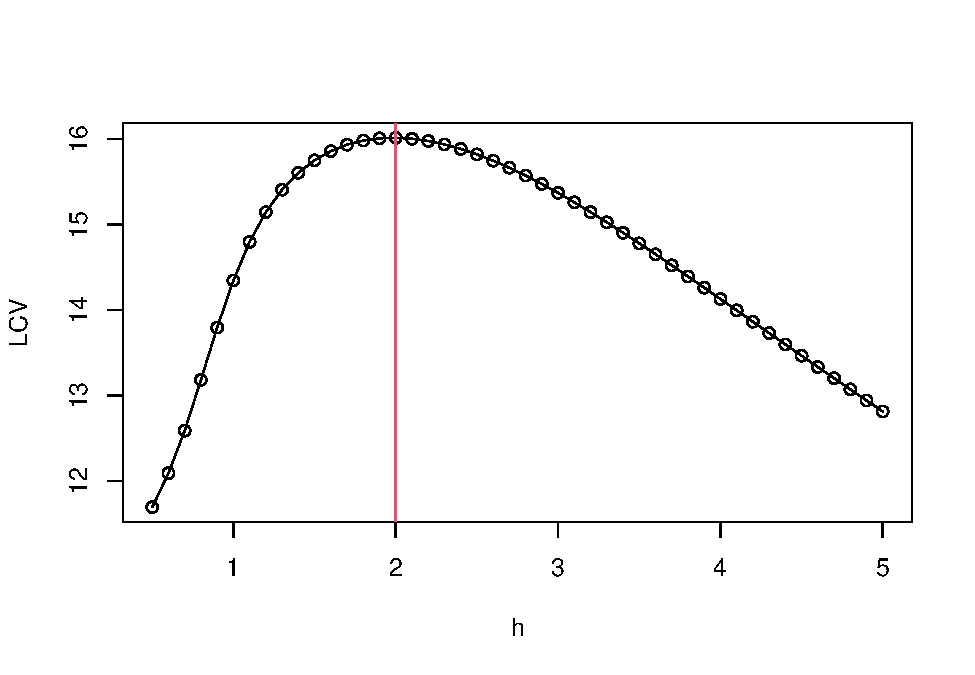
\includegraphics{Problemsetrmd_files/figure-latex/unnamed-chunk-4-1.pdf}

\begin{verbatim}
## integer(0)
\end{verbatim}

\begin{Shaded}
\begin{Highlighting}[]
\NormalTok{h[}\FunctionTok{which.max}\NormalTok{(LCV)]}
\end{Highlighting}
\end{Shaded}

\begin{verbatim}
## [1] 2
\end{verbatim}

For this section we have used the function that computes the Least Cross
Validation bandwidth estimator through likelihood cross validation. The
function basically minimizes the regression model thanks to the nlm()
function, using p=c(0,0) as a starting point. Both the plot and the
h{[}which.max(LCV){]} return an estimation of h=2 (relatively close to
the somehow adequate h=1.5 that we used in the previous section).

\hypertarget{c.-using-hlcv-predict-the-probability-of-an-incident-at-temperatures-0.6-launch-temperature-of-the-challenger-and-11.67-specific-recommendation-by-the-vice-president-of-engineers.}{%
\subsubsection{c.~Using hLCV, predict the probability of an incident at
temperatures −0.6 (launch temperature of the Challenger) and 11.67
(specific recommendation by the vice president of
engineers).}\label{c.-using-hlcv-predict-the-probability-of-an-incident-at-temperatures-0.6-launch-temperature-of-the-challenger-and-11.67-specific-recommendation-by-the-vice-president-of-engineers.}}

\begin{Shaded}
\begin{Highlighting}[]
\NormalTok{hlcv }\OtherTok{\textless{}{-}} \DecValTok{2}
\NormalTok{fit\_locfit\_lcv }\OtherTok{\textless{}{-}}\NormalTok{ locfit}\SpecialCharTok{::}\FunctionTok{locfit}\NormalTok{(Y }\SpecialCharTok{\textasciitilde{}}\NormalTok{ locfit}\SpecialCharTok{::}\FunctionTok{lp}\NormalTok{(X, }\AttributeTok{deg =} \DecValTok{1}\NormalTok{, }\AttributeTok{nn =}\NormalTok{ hlcv),}
                             \AttributeTok{family =} \StringTok{"binomial"}\NormalTok{, }\AttributeTok{kern =} \StringTok{"gauss"}\NormalTok{)}
\NormalTok{prediction }\OtherTok{\textless{}{-}} \FunctionTok{predict}\NormalTok{(fit\_locfit\_lcv, }\FunctionTok{c}\NormalTok{(}\SpecialCharTok{{-}}\FloatTok{0.6}\NormalTok{,}\FloatTok{11.67}\NormalTok{))}
\NormalTok{prediction}
\end{Highlighting}
\end{Shaded}

\begin{verbatim}
## [1] 0.9998206 0.9535512
\end{verbatim}

We have obtained probabilities of 0.9998206 and 0.9535512 respectively
for -0.6 and 11.67 degrees. Obviously, it is highly probable to have an
incident with any of these temperatures. If we take a look at the plot
of the regression model, we can see that, for temperatures under
approximately 15 degrees, the response variable will always return ``1''
as the outcome, i.e., an incident occurring. Therefore, it holds that
the probabilities obtained for such low temperatures are these high.

\hypertarget{d.-what-are-the-local-odds-at-0.6-and-11.67-show-the-local-logistic-models-about-these-points-in-spirit-of-figure-5.1-and-interpret-the-results.}{%
\subsubsection{d.~What are the local odds at −0.6 and 11.67? Show the
local logistic models about these points, in spirit of Figure 5.1, and
interpret the
results.}\label{d.-what-are-the-local-odds-at-0.6-and-11.67-show-the-local-logistic-models-about-these-points-in-spirit-of-figure-5.1-and-interpret-the-results.}}

Now, we can compute the local odds as follows:

\begin{Shaded}
\begin{Highlighting}[]
\NormalTok{local\_odds1 }\OtherTok{\textless{}{-}}\NormalTok{ prediction[}\DecValTok{1}\NormalTok{]}\SpecialCharTok{/}\NormalTok{(}\DecValTok{1}\SpecialCharTok{{-}}\NormalTok{prediction[}\DecValTok{1}\NormalTok{])}
\NormalTok{local\_odds1}
\end{Highlighting}
\end{Shaded}

\begin{verbatim}
## [1] 5573.327
\end{verbatim}

\begin{Shaded}
\begin{Highlighting}[]
\NormalTok{local\_odds2 }\OtherTok{\textless{}{-}}\NormalTok{ prediction[}\DecValTok{2}\NormalTok{]}\SpecialCharTok{/}\NormalTok{(}\DecValTok{1}\SpecialCharTok{{-}}\NormalTok{prediction[}\DecValTok{2}\NormalTok{])}
\NormalTok{local\_odds2}
\end{Highlighting}
\end{Shaded}

\begin{verbatim}
## [1] 20.52908
\end{verbatim}

In order to show the local logistic model for these points, we need to
give a different approach to implement the logistic models, this time
using glm.fit().

First, we use X=-0.6 and Y=1.

\begin{Shaded}
\begin{Highlighting}[]
\NormalTok{logistic }\OtherTok{\textless{}{-}} \ControlFlowTok{function}\NormalTok{(x) }\DecValTok{1} \SpecialCharTok{/}\NormalTok{ (}\DecValTok{1} \SpecialCharTok{+} \FunctionTok{exp}\NormalTok{(}\SpecialCharTok{{-}}\NormalTok{x))}
\NormalTok{Xev }\OtherTok{=} \SpecialCharTok{{-}}\FloatTok{0.6}
\NormalTok{Yev}\OtherTok{=}\DecValTok{1}
\NormalTok{x }\OtherTok{=} \FunctionTok{seq}\NormalTok{(}\SpecialCharTok{{-}}\DecValTok{3}\NormalTok{, }\DecValTok{40}\NormalTok{, }\AttributeTok{by =} \FloatTok{0.1}\NormalTok{)}
\FunctionTok{suppressWarnings}\NormalTok{(}
\NormalTok{  fit\_nlm\_local1 }\OtherTok{\textless{}{-}} \FunctionTok{sapply}\NormalTok{(x, }\ControlFlowTok{function}\NormalTok{(x) \{}
\NormalTok{    K }\OtherTok{\textless{}{-}} \FunctionTok{dnorm}\NormalTok{(}\AttributeTok{x =}\NormalTok{ x, }\AttributeTok{mean =}\NormalTok{ Xev, }\AttributeTok{sd =} \FloatTok{1.9}\NormalTok{)}
    \FunctionTok{nlm}\NormalTok{(}\AttributeTok{f =} \ControlFlowTok{function}\NormalTok{(beta) \{}
      \SpecialCharTok{{-}}\FunctionTok{sum}\NormalTok{(K }\SpecialCharTok{*}\NormalTok{ (Yev }\SpecialCharTok{*}\NormalTok{ (beta[}\DecValTok{1}\NormalTok{] }\SpecialCharTok{+}\NormalTok{ beta[}\DecValTok{2}\NormalTok{] }\SpecialCharTok{*}\NormalTok{ (Xev }\SpecialCharTok{{-}}\NormalTok{ x)) }\SpecialCharTok{{-}}
                  \FunctionTok{log}\NormalTok{(}\DecValTok{1} \SpecialCharTok{+} \FunctionTok{exp}\NormalTok{(beta[}\DecValTok{1}\NormalTok{] }\SpecialCharTok{+}\NormalTok{ beta[}\DecValTok{2}\NormalTok{] }\SpecialCharTok{*}\NormalTok{ (Xev }\SpecialCharTok{{-}}\NormalTok{ x)))))}
\NormalTok{    \}, }\AttributeTok{p =} \FunctionTok{c}\NormalTok{(}\DecValTok{0}\NormalTok{, }\DecValTok{0}\NormalTok{))}\SpecialCharTok{$}\NormalTok{estimate[}\DecValTok{1}\NormalTok{]}
\NormalTok{  \})}
\NormalTok{)}
\FunctionTok{plot}\NormalTok{(x,}\FunctionTok{logistic}\NormalTok{(fit\_nlm\_local1), }\AttributeTok{type=}\StringTok{"l"}\NormalTok{, }\AttributeTok{xlim =} \FunctionTok{c}\NormalTok{(}\DecValTok{0}\NormalTok{,}\DecValTok{30}\NormalTok{)) }\SpecialCharTok{+} \FunctionTok{plot}\NormalTok{(fit\_locfit\_lcv, }\AttributeTok{xlim =} \FunctionTok{c}\NormalTok{(}\SpecialCharTok{{-}}\DecValTok{1}\NormalTok{,}\DecValTok{28}\NormalTok{))}
\end{Highlighting}
\end{Shaded}

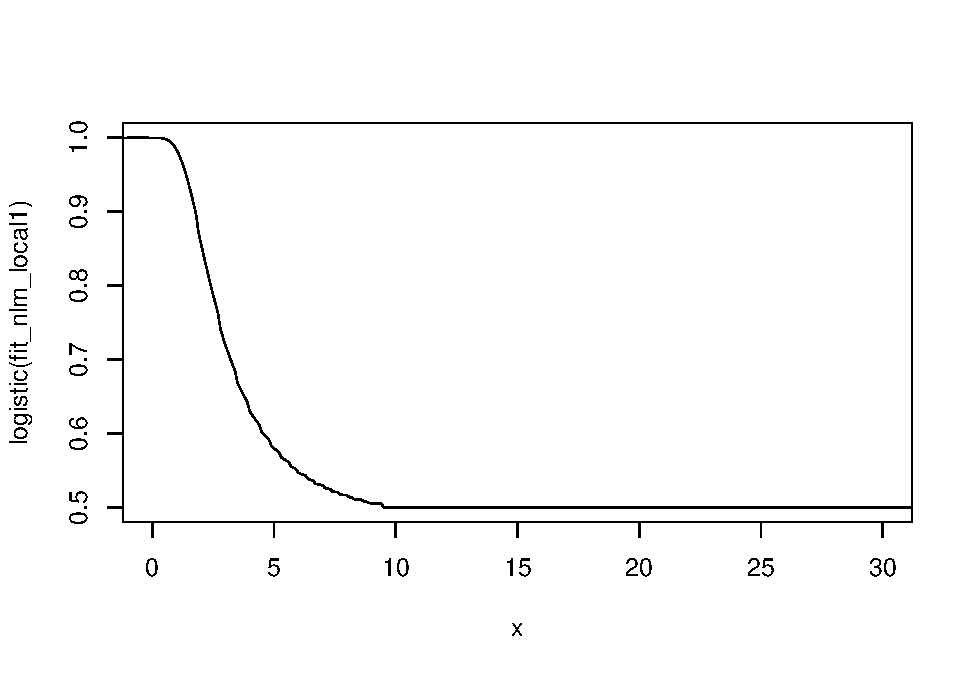
\includegraphics{Problemsetrmd_files/figure-latex/unnamed-chunk-7-1.pdf}
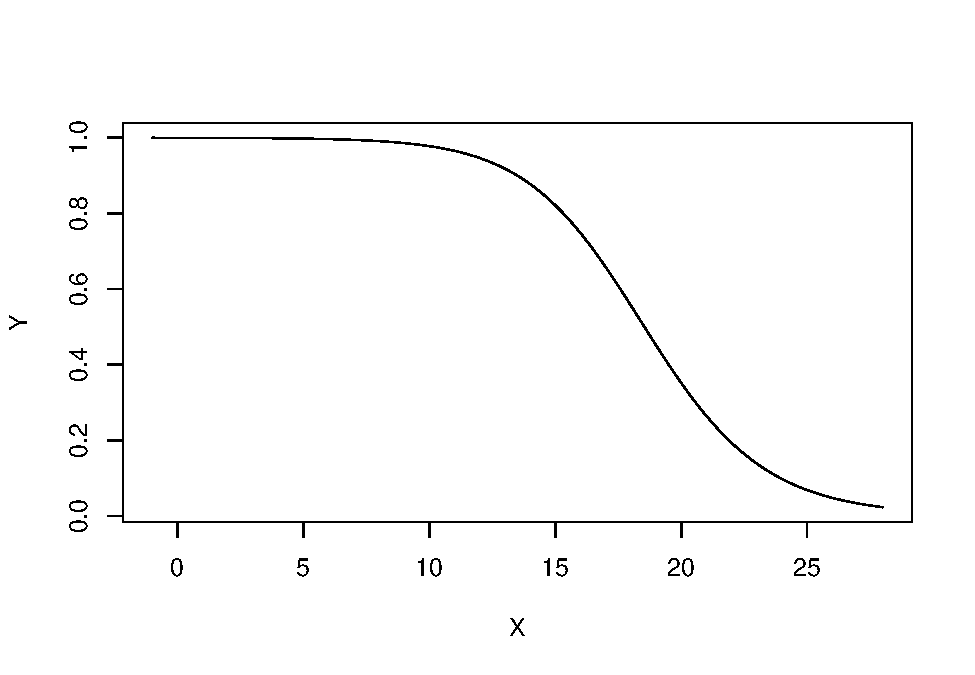
\includegraphics{Problemsetrmd_files/figure-latex/unnamed-chunk-7-2.pdf}

\begin{verbatim}
## integer(0)
\end{verbatim}

Now, the same but with X = 1.67 and Y = 1.

\begin{Shaded}
\begin{Highlighting}[]
\NormalTok{Xev2 }\OtherTok{\textless{}{-}} \FloatTok{11.67}
\NormalTok{logistic }\OtherTok{\textless{}{-}} \ControlFlowTok{function}\NormalTok{(x) }\DecValTok{1} \SpecialCharTok{/}\NormalTok{ (}\DecValTok{1} \SpecialCharTok{+} \FunctionTok{exp}\NormalTok{(}\SpecialCharTok{{-}}\NormalTok{x))}
\NormalTok{Yev}\OtherTok{=}\DecValTok{1}
\NormalTok{x }\OtherTok{=} \FunctionTok{seq}\NormalTok{(}\FunctionTok{min}\NormalTok{(X), }\FunctionTok{max}\NormalTok{(X), }\AttributeTok{by =} \FloatTok{0.1}\NormalTok{)}
\FunctionTok{suppressWarnings}\NormalTok{(}
\NormalTok{  fit\_nlm\_local2 }\OtherTok{\textless{}{-}} \FunctionTok{sapply}\NormalTok{(x, }\ControlFlowTok{function}\NormalTok{(x) \{}
\NormalTok{    K }\OtherTok{\textless{}{-}} \FunctionTok{dnorm}\NormalTok{(}\AttributeTok{x =}\NormalTok{ x, }\AttributeTok{mean =}\NormalTok{ Xev2, }\AttributeTok{sd =} \DecValTok{2}\NormalTok{)}
    \FunctionTok{nlm}\NormalTok{(}\AttributeTok{f =} \ControlFlowTok{function}\NormalTok{(beta) \{}
      \SpecialCharTok{{-}}\FunctionTok{sum}\NormalTok{(K }\SpecialCharTok{*}\NormalTok{ (Yev }\SpecialCharTok{*}\NormalTok{ (beta[}\DecValTok{1}\NormalTok{] }\SpecialCharTok{+}\NormalTok{ beta[}\DecValTok{2}\NormalTok{] }\SpecialCharTok{*}\NormalTok{ (Xev2 }\SpecialCharTok{{-}}\NormalTok{ x)) }\SpecialCharTok{{-}}
                  \FunctionTok{log}\NormalTok{(}\DecValTok{1} \SpecialCharTok{+} \FunctionTok{exp}\NormalTok{(beta[}\DecValTok{1}\NormalTok{] }\SpecialCharTok{+}\NormalTok{ beta[}\DecValTok{2}\NormalTok{] }\SpecialCharTok{*}\NormalTok{ (Xev2 }\SpecialCharTok{{-}}\NormalTok{ x)))))}
\NormalTok{    \}, }\AttributeTok{p =} \FunctionTok{c}\NormalTok{(}\DecValTok{0}\NormalTok{, }\DecValTok{0}\NormalTok{))}\SpecialCharTok{$}\NormalTok{estimate[}\DecValTok{1}\NormalTok{]}
\NormalTok{  \})}
\NormalTok{)}

\FunctionTok{plot}\NormalTok{(fit\_locfit\_lcv, }\AttributeTok{col =} \DecValTok{4}\NormalTok{) }\SpecialCharTok{+} \FunctionTok{plot}\NormalTok{(x,}\FunctionTok{logistic}\NormalTok{(fit\_nlm\_local2), }\AttributeTok{col=}\DecValTok{2}\NormalTok{, }\AttributeTok{type=}\StringTok{"l"}\NormalTok{) }
\end{Highlighting}
\end{Shaded}

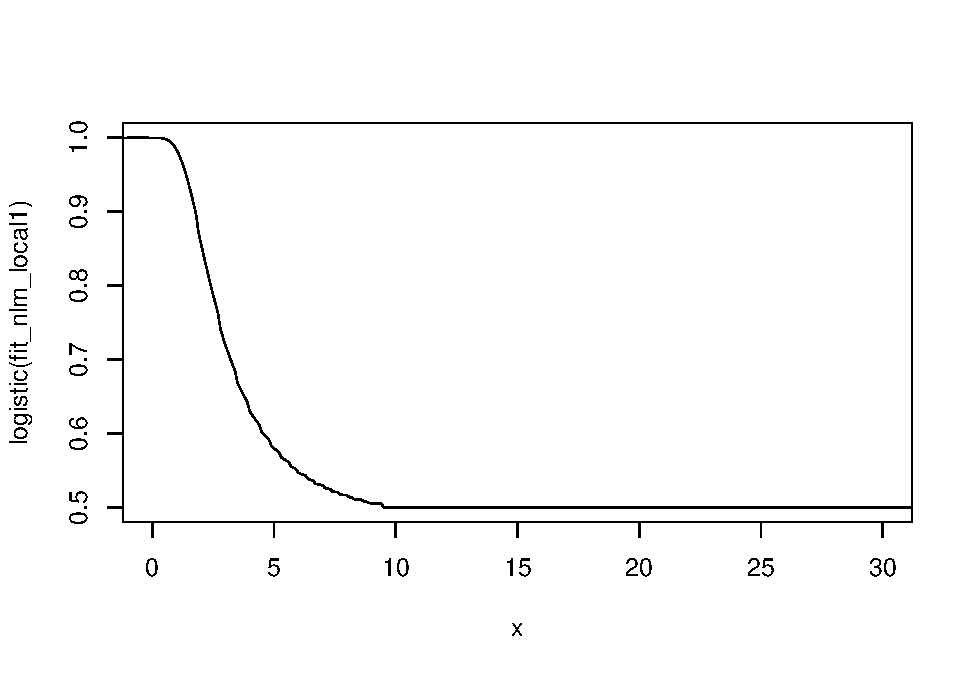
\includegraphics{Problemsetrmd_files/figure-latex/unnamed-chunk-8-1.pdf}
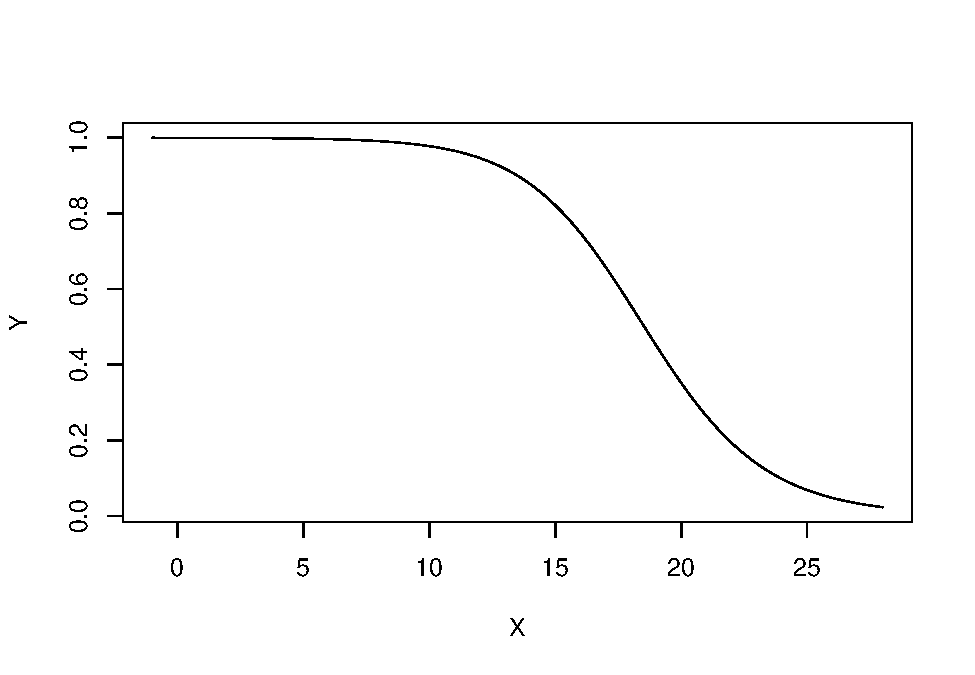
\includegraphics{Problemsetrmd_files/figure-latex/unnamed-chunk-8-2.pdf}

\begin{verbatim}
## integer(0)
\end{verbatim}

Thanks to all these plots we can see that, as in Figure 5.1, the local
logistic estimated model for the points evaluated and the points in the
original plots coincide, which is what we were looking for.

\hypertarget{exercise-4.9.-perform-the-following-tasks}{%
\subsection{Exercise 4.9. Perform the following
tasks:}\label{exercise-4.9.-perform-the-following-tasks}}

\hypertarget{a.-code-your-own-implementation-of-the-local-cubic-estimator.-the-function-must-take-as-input-the-vector-of-evaluation-points-x-the-sample-data-and-the-bandwidth-h.-use-the-normal-kernel.-the-result-must-be-a-vector-of-the-same-length-as-x-containing-the-estimator-evaluated-at-x.}{%
\subsubsection{a. Code your own implementation of the local cubic
estimator. The function must take as input the vector of evaluation
points x, the sample data, and the bandwidth h. Use the normal kernel.
The result must be a vector of the same length as x containing the
estimator evaluated at
x.}\label{a.-code-your-own-implementation-of-the-local-cubic-estimator.-the-function-must-take-as-input-the-vector-of-evaluation-points-x-the-sample-data-and-the-bandwidth-h.-use-the-normal-kernel.-the-result-must-be-a-vector-of-the-same-length-as-x-containing-the-estimator-evaluated-at-x.}}

For this exercise, we have used the derivation of a general local linear
estimator (for any p). From there, we have implemented the equations
needed to obtain the local cubic estimator. These equations result
mainly from the multiplication of the matrices X, W and Y and we had to
create them.

In the creation of the matrix X, we have fixed the value p=3 and
computed the matrix. After that, inside the same loop (from 1 to the
length of the vector of evaluation points), we created the diagonal
matrix W and the final estimation obtained from the multiplication of
the matrices (and the multiplication of t(e1) at the beginning of the
calculations in order to keep just the first row).

\begin{Shaded}
\begin{Highlighting}[]
\FunctionTok{set.seed}\NormalTok{(}\DecValTok{1233}\NormalTok{)}

\NormalTok{local\_cubic}\OtherTok{=}\ControlFlowTok{function}\NormalTok{(DF,x,h)\{}
\NormalTok{  X}\OtherTok{=}\FunctionTok{matrix}\NormalTok{(}\AttributeTok{nrow=}\FunctionTok{nrow}\NormalTok{(DF),}\AttributeTok{ncol=}\DecValTok{4}\NormalTok{)}
\NormalTok{  estim\_x}\OtherTok{=}\FunctionTok{c}\NormalTok{()}
  \ControlFlowTok{for}\NormalTok{ (i }\ControlFlowTok{in} \DecValTok{1}\SpecialCharTok{:}\FunctionTok{length}\NormalTok{(x)) \{}
    \ControlFlowTok{for}\NormalTok{(p }\ControlFlowTok{in} \DecValTok{0}\SpecialCharTok{:}\DecValTok{3}\NormalTok{)\{}
\NormalTok{        X[,(p}\SpecialCharTok{+}\DecValTok{1}\NormalTok{)]}\OtherTok{=}\NormalTok{(DF}\SpecialCharTok{$}\NormalTok{X}\SpecialCharTok{{-}}\NormalTok{x[i])}\SpecialCharTok{\^{}}\NormalTok{p}
\NormalTok{    \}}
\NormalTok{    W}\OtherTok{=}\FunctionTok{diag}\NormalTok{(}\FunctionTok{dnorm}\NormalTok{(DF}\SpecialCharTok{$}\NormalTok{X}\SpecialCharTok{{-}}\NormalTok{x[i]}\SpecialCharTok{/}\NormalTok{h)}\SpecialCharTok{/}\NormalTok{h)}
\NormalTok{    estim\_x[i]}\OtherTok{=} \FunctionTok{t}\NormalTok{(}\FunctionTok{c}\NormalTok{(}\DecValTok{1}\NormalTok{,}\DecValTok{0}\NormalTok{,}\DecValTok{0}\NormalTok{,}\DecValTok{0}\NormalTok{)) }\SpecialCharTok{\%*\%}\NormalTok{ (}\FunctionTok{t}\NormalTok{(X)}\SpecialCharTok{\%*\%}\NormalTok{W}\SpecialCharTok{\%*\%}\NormalTok{X }\SpecialCharTok{\%\textgreater{}\%} \FunctionTok{ginv}\NormalTok{()) }\SpecialCharTok{\%*\%}\NormalTok{ (}\FunctionTok{t}\NormalTok{(X) }\SpecialCharTok{\%*\%}\NormalTok{ W }\SpecialCharTok{\%*\%}\NormalTok{ DF}\SpecialCharTok{$}\NormalTok{Y) }
\NormalTok{  \}}
  
  \FunctionTok{return}\NormalTok{(estim\_x)}
\NormalTok{\}}
\end{Highlighting}
\end{Shaded}

We created a data frame with the variables X and Y. After that, we
implemented the function and plotted the results to see how good the
estimation is.

\begin{Shaded}
\begin{Highlighting}[]
\NormalTok{n}\OtherTok{=}\DecValTok{500}
\NormalTok{X}\OtherTok{=}\FunctionTok{rnorm}\NormalTok{(n,}\DecValTok{1}\NormalTok{,}\DecValTok{1}\NormalTok{)}
\NormalTok{x}\OtherTok{=}\FunctionTok{seq}\NormalTok{(}\SpecialCharTok{{-}}\DecValTok{4}\NormalTok{,}\DecValTok{4}\NormalTok{,}\AttributeTok{l=}\DecValTok{600}\NormalTok{)}

\NormalTok{m}\OtherTok{=}\ControlFlowTok{function}\NormalTok{(x)\{}
  \FunctionTok{return}\NormalTok{((x}\DecValTok{{-}1}\NormalTok{)}\SpecialCharTok{\^{}}\DecValTok{2}\NormalTok{)}
\NormalTok{\}}

\NormalTok{err}\OtherTok{=}\FunctionTok{rnorm}\NormalTok{(n,}\DecValTok{0}\NormalTok{,}\FloatTok{0.5}\NormalTok{)}

\NormalTok{Y}\OtherTok{=}\FunctionTok{m}\NormalTok{(X)}\SpecialCharTok{+}\NormalTok{err}
\NormalTok{DF}\OtherTok{=}\FunctionTok{data.frame}\NormalTok{(X,Y)}


\NormalTok{Te}\OtherTok{=}\FunctionTok{local\_cubic}\NormalTok{(DF,x,h)}
\NormalTok{m}\OtherTok{=}\FunctionTok{m}\NormalTok{(x)}

\FunctionTok{ggplot}\NormalTok{() }\SpecialCharTok{+} \FunctionTok{geom\_point}\NormalTok{(}\AttributeTok{data =}\NormalTok{ DF,}\FunctionTok{aes}\NormalTok{(}\AttributeTok{x=}\NormalTok{X,}\AttributeTok{y=}\NormalTok{Y),}\AttributeTok{shape=}\DecValTok{1}\NormalTok{) }\SpecialCharTok{+} \FunctionTok{geom\_line}\NormalTok{(}\FunctionTok{aes}\NormalTok{(x,m),}\AttributeTok{col=}\StringTok{"4"}\NormalTok{) }\SpecialCharTok{+} 
  \FunctionTok{geom\_line}\NormalTok{(}\FunctionTok{aes}\NormalTok{(x,Te),}\AttributeTok{col=}\StringTok{"2"}\NormalTok{) }\SpecialCharTok{+} \FunctionTok{xlim}\NormalTok{(}\SpecialCharTok{{-}}\DecValTok{3}\NormalTok{,}\DecValTok{4}\NormalTok{) }\SpecialCharTok{+} \FunctionTok{ylim}\NormalTok{(}\SpecialCharTok{{-}}\DecValTok{2}\NormalTok{,}\DecValTok{8}\NormalTok{)}
\end{Highlighting}
\end{Shaded}

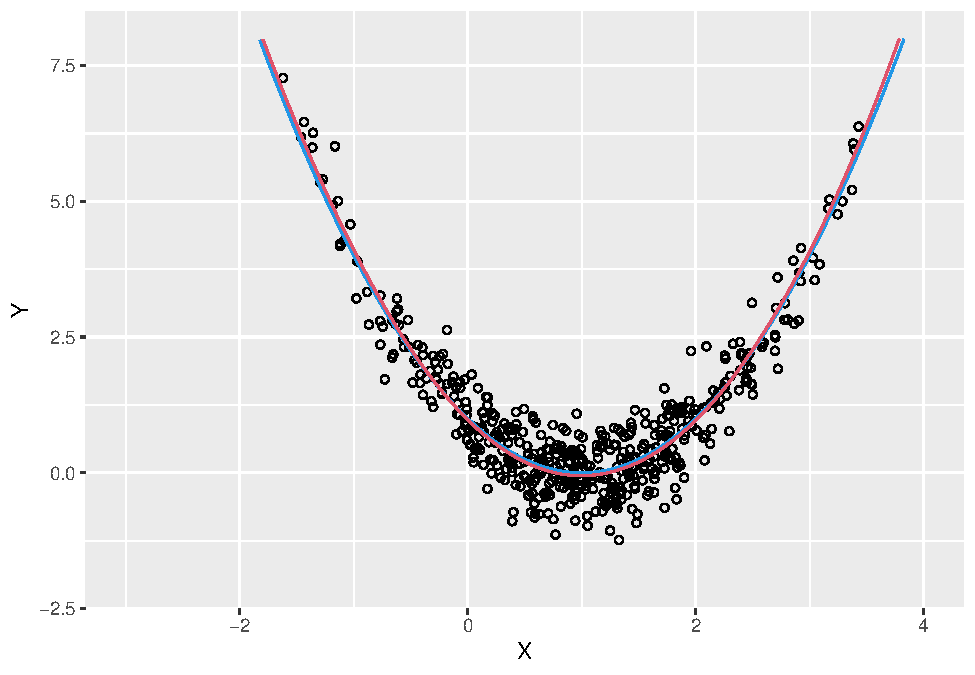
\includegraphics{Problemsetrmd_files/figure-latex/unnamed-chunk-10-1.pdf}

First, we plotted the estimated regression function of the evaluation
points. After that, we added the real function m applied to the
evaluation points and the estimation of this function. We can clearly
see that the estimation of m(x) (m(x,3,h)) is quite accurate, since it
is very similar to the real m(x) and follows the same path as the
estimated regression function.

\hypertarget{exercise-3.31.-implement-the-euler-method-for-f-being-f_oval-f_croissant-and-f_sin-in-order-to-reproduce-figure-3.18.}{%
\subsection{Exercise 3.31. Implement the Euler method for f being
f\_oval, f\_croissant, and f\_sin, in order to reproduce Figure
3.18.}\label{exercise-3.31.-implement-the-euler-method-for-f-being-f_oval-f_croissant-and-f_sin-in-order-to-reproduce-figure-3.18.}}

Let's implement the whole exercise for the function f\_oval first and
then adapt it to the rest of the functions. Of course, we start by
computing this function.

\begin{Shaded}
\begin{Highlighting}[]
\CommentTok{\# Our functions }

\CommentTok{\# "Oval" density}
\NormalTok{f\_oval }\OtherTok{\textless{}{-}} \ControlFlowTok{function}\NormalTok{(x, }\AttributeTok{mu =} \DecValTok{2}\NormalTok{, }\AttributeTok{sigma =} \FloatTok{0.35}\NormalTok{, }
                   \AttributeTok{Sigma =} \FunctionTok{rbind}\NormalTok{(}\FunctionTok{c}\NormalTok{(}\DecValTok{1}\NormalTok{, }\SpecialCharTok{{-}}\FloatTok{0.71}\NormalTok{), }\FunctionTok{c}\NormalTok{(}\SpecialCharTok{{-}}\FloatTok{0.71}\NormalTok{, }\DecValTok{2}\NormalTok{))) \{}
  
  \CommentTok{\# x always as a matrix}
\NormalTok{  x }\OtherTok{\textless{}{-}} \FunctionTok{rbind}\NormalTok{(x)}
  
  \CommentTok{\# Rotate x with distortion}
\NormalTok{  Sigma\_inv\_sqrt }\OtherTok{\textless{}{-}} \FunctionTok{solve}\NormalTok{(}\FunctionTok{chol}\NormalTok{(Sigma))}
\NormalTok{  x }\OtherTok{\textless{}{-}}\NormalTok{ x }\SpecialCharTok{\%*\%}\NormalTok{ Sigma\_inv\_sqrt}
  
  \CommentTok{\# Polar coordinates}
\NormalTok{  r }\OtherTok{\textless{}{-}} \FunctionTok{sqrt}\NormalTok{(}\FunctionTok{rowSums}\NormalTok{(x}\SpecialCharTok{\^{}}\DecValTok{2}\NormalTok{))}
  
  \CommentTok{\# Density as conditional * marginal}
\NormalTok{  f\_theta }\OtherTok{\textless{}{-}} \DecValTok{1} \SpecialCharTok{/}\NormalTok{ (}\DecValTok{2} \SpecialCharTok{*}\NormalTok{ pi)}
\NormalTok{  f\_r\_theta }\OtherTok{\textless{}{-}} \FunctionTok{dnorm}\NormalTok{(}\AttributeTok{x =}\NormalTok{ r, }\AttributeTok{mean =}\NormalTok{ mu, }\AttributeTok{sd =}\NormalTok{ sigma)}
\NormalTok{  jacobian }\OtherTok{\textless{}{-}}  \FunctionTok{det}\NormalTok{(Sigma\_inv\_sqrt) }\SpecialCharTok{/}\NormalTok{ r}
\NormalTok{  f }\OtherTok{\textless{}{-}}\NormalTok{ f\_r\_theta }\SpecialCharTok{*}\NormalTok{ f\_theta }\SpecialCharTok{*}\NormalTok{ jacobian}
  \FunctionTok{return}\NormalTok{(f)}
  
\NormalTok{\}}
\end{Highlighting}
\end{Shaded}

Now, we have to implement the projection of the gradient into the
Hessian s-th eigenvector subspace. In order to do so, we have made a few
changes to the original function.

First of all, we have used the functions numDeriv::grad and
numDeriv::hessian in order to obtain the gradient and the hessian of the
function. Since the objects return from these functions were not the
same as the ones from the grad\_norm() and hess\_norm() functions used
before, we had to adjust them in order to make the main function work.
For instance, the object grad was not a matrix at the beginning and,
therefore, we could not choose the elements grad{[}i,{]}, so we had to
adjust this. A few other variations were made and they can be seen in
the function:

\begin{Shaded}
\begin{Highlighting}[]
\CommentTok{\# Projected gradient into the Hessian s{-}th eigenvector subspace}
\NormalTok{proj\_grad\_norm\_oval }\OtherTok{\textless{}{-}} \ControlFlowTok{function}\NormalTok{(x, mu, Sigma, }\AttributeTok{s =} \DecValTok{2}\NormalTok{) \{}
  
  \CommentTok{\# Gradient}
\NormalTok{  grad }\OtherTok{\textless{}{-}}\NormalTok{ numDeriv}\SpecialCharTok{::}\FunctionTok{grad}\NormalTok{(f\_oval,x) }\SpecialCharTok{\%\textgreater{}\%} \FunctionTok{as.matrix}\NormalTok{() }\SpecialCharTok{\%\textgreater{}\%} \FunctionTok{t}\NormalTok{()}
  
  \CommentTok{\# Hessian}
\NormalTok{  Hess }\OtherTok{\textless{}{-}}\NormalTok{ numDeriv}\SpecialCharTok{::}\FunctionTok{hessian}\NormalTok{(f\_oval,x)}
  
  \CommentTok{\# Eigenvectors Hessian}
\NormalTok{  eig\_Hess }\OtherTok{\textless{}{-}} \ControlFlowTok{function}\NormalTok{(A)\{}
    \FunctionTok{t}\NormalTok{(}\FunctionTok{as.matrix}\NormalTok{(}\FunctionTok{eigen}\NormalTok{(}\AttributeTok{x =}\NormalTok{ A, }\AttributeTok{symmetric =} \ConstantTok{TRUE}\NormalTok{)}\SpecialCharTok{$}\NormalTok{vectors[, s]))}
\NormalTok{  \} }
\NormalTok{  eig\_hess }\OtherTok{\textless{}{-}} \FunctionTok{eig\_Hess}\NormalTok{(Hess)}
  
  \CommentTok{\# Projected gradient}
\NormalTok{  proj\_grad }\OtherTok{\textless{}{-}} \FunctionTok{t}\NormalTok{(}\FunctionTok{sapply}\NormalTok{(}\DecValTok{1}\SpecialCharTok{:}\FunctionTok{nrow}\NormalTok{(eig\_hess), }\ControlFlowTok{function}\NormalTok{(i) \{}
    \FunctionTok{tcrossprod}\NormalTok{(eig\_hess[i,]) }\SpecialCharTok{\%*\%}\NormalTok{ grad[i,]}
\NormalTok{  \}))}
  
  \CommentTok{\# As an array}
  \FunctionTok{return}\NormalTok{(proj\_grad)}
  
\NormalTok{\}}
\end{Highlighting}
\end{Shaded}

Now, we had to implement the main function for the Euler solution. Here,
we had some constraints that stopped the iteration if
\(\|x_{t+1} − x_{t}\|_{\infty} < \epsilon \hspace{0.2cm} or \hspace{0.2cm} \|x_{t+1} − x_{t}\|_{\infty}/\|x_{t}\|_{\infty} < \epsilon\),
but we added another constraint that disregarded the final points if
\(f(x) < 50*\delta\). For this, we implemented this constraint before
plotting the final points, allowing to plot the points that only satisfy
this constraint.

\begin{Shaded}
\begin{Highlighting}[]
\CommentTok{\# Euler solution}
\FunctionTok{plot}\NormalTok{(}\AttributeTok{x=}\DecValTok{1}\NormalTok{,}\AttributeTok{y=}\DecValTok{1}\NormalTok{, }\AttributeTok{xlim=}\FunctionTok{c}\NormalTok{(}\SpecialCharTok{{-}}\DecValTok{4}\NormalTok{,}\DecValTok{4}\NormalTok{), }\AttributeTok{ylim=}\FunctionTok{c}\NormalTok{(}\SpecialCharTok{{-}}\DecValTok{4}\NormalTok{,}\DecValTok{4}\NormalTok{))}
\NormalTok{x0 }\OtherTok{\textless{}{-}} \FunctionTok{as.matrix}\NormalTok{(}\FunctionTok{expand.grid}\NormalTok{(}\FunctionTok{seq}\NormalTok{(}\SpecialCharTok{{-}}\DecValTok{3}\NormalTok{, }\DecValTok{3}\NormalTok{, }\AttributeTok{l =} \DecValTok{12}\NormalTok{), }\FunctionTok{seq}\NormalTok{(}\SpecialCharTok{{-}}\DecValTok{3}\NormalTok{, }\DecValTok{3}\NormalTok{, }\AttributeTok{l =} \DecValTok{12}\NormalTok{)))}
\NormalTok{x }\OtherTok{\textless{}{-}} \FunctionTok{matrix}\NormalTok{(}\ConstantTok{NA}\NormalTok{, }\AttributeTok{nrow =} \FunctionTok{nrow}\NormalTok{(x0), }\AttributeTok{ncol =} \DecValTok{2}\NormalTok{)}
\NormalTok{N }\OtherTok{\textless{}{-}} \DecValTok{100}
\NormalTok{h }\OtherTok{\textless{}{-}} \FloatTok{0.06}
\NormalTok{phi }\OtherTok{\textless{}{-}} \FunctionTok{matrix}\NormalTok{(}\AttributeTok{nrow =}\NormalTok{ N }\SpecialCharTok{+} \DecValTok{1}\NormalTok{, }\AttributeTok{ncol =} \DecValTok{2}\NormalTok{)}
\NormalTok{eps }\OtherTok{\textless{}{-}} \FloatTok{1e{-}4}
\NormalTok{mu }\OtherTok{\textless{}{-}} \FunctionTok{c}\NormalTok{(}\DecValTok{0}\NormalTok{,}\DecValTok{0}\NormalTok{)}
\NormalTok{Sigma }\OtherTok{\textless{}{-}} \FunctionTok{rbind}\NormalTok{(}\FunctionTok{c}\NormalTok{(}\DecValTok{1}\NormalTok{, }\SpecialCharTok{{-}}\FloatTok{0.71}\NormalTok{), }\FunctionTok{c}\NormalTok{(}\SpecialCharTok{{-}}\FloatTok{0.71}\NormalTok{, }\DecValTok{2}\NormalTok{))}
\NormalTok{delta }\OtherTok{\textless{}{-}} \DecValTok{1}\NormalTok{.e}\DecValTok{{-}3}
\NormalTok{count}\OtherTok{=}\DecValTok{0}

\ControlFlowTok{for}\NormalTok{ (i }\ControlFlowTok{in} \DecValTok{1}\SpecialCharTok{:}\FunctionTok{nrow}\NormalTok{(x0)) \{}
  
  \CommentTok{\# Move along the flow curve}
\NormalTok{  phi[}\DecValTok{1}\NormalTok{, ] }\OtherTok{\textless{}{-}}\NormalTok{ x0[i, ]}
  \ControlFlowTok{for}\NormalTok{ (t }\ControlFlowTok{in} \DecValTok{1}\SpecialCharTok{:}\NormalTok{N) \{}
    
    \CommentTok{\# Euler update}
\NormalTok{      phi[t }\SpecialCharTok{+} \DecValTok{1}\NormalTok{, ] }\OtherTok{\textless{}{-}}\NormalTok{ phi[t, ] }\SpecialCharTok{+} 
\NormalTok{        h }\SpecialCharTok{*} \FunctionTok{proj\_grad\_norm\_oval}\NormalTok{(phi[t, ], }\AttributeTok{mu =}\NormalTok{ mu, }\AttributeTok{Sigma =}\NormalTok{ Sigma) }\SpecialCharTok{/}
        \FunctionTok{f\_oval}\NormalTok{(}\AttributeTok{x =}\NormalTok{ phi[t, ])}
      
      \CommentTok{\# Stopping criterion (to save computing time!)}
\NormalTok{      abs\_tol }\OtherTok{\textless{}{-}} \FunctionTok{max}\NormalTok{(}\FunctionTok{abs}\NormalTok{(phi[t }\SpecialCharTok{+} \DecValTok{1}\NormalTok{, ] }\SpecialCharTok{{-}}\NormalTok{ phi[t, ]))}
\NormalTok{      rel\_tol }\OtherTok{\textless{}{-}}\NormalTok{ abs\_tol }\SpecialCharTok{/} \FunctionTok{max}\NormalTok{(}\FunctionTok{abs}\NormalTok{(phi[t, ]))}
      \ControlFlowTok{if}\NormalTok{ (abs\_tol }\SpecialCharTok{\textless{}}\NormalTok{ eps }\SpecialCharTok{|}\NormalTok{ rel\_tol }\SpecialCharTok{\textless{}}\NormalTok{ eps) }\ControlFlowTok{break}
      
\NormalTok{  \}}
  
  \CommentTok{\# Save final point}
\NormalTok{  x[i, ] }\OtherTok{\textless{}{-}}\NormalTok{ phi[t }\SpecialCharTok{+} \DecValTok{1}\NormalTok{, , drop }\OtherTok{=} \ConstantTok{FALSE}\NormalTok{]}

    
  \CommentTok{\# Plot lines and x0}
  \FunctionTok{lines}\NormalTok{(phi[}\DecValTok{1}\SpecialCharTok{:}\NormalTok{(t }\SpecialCharTok{+} \DecValTok{1}\NormalTok{), ], }\AttributeTok{type =} \StringTok{"l"}\NormalTok{) }
  \FunctionTok{points}\NormalTok{(x0[i, , }\AttributeTok{drop =} \ConstantTok{FALSE}\NormalTok{], }\AttributeTok{pch =} \DecValTok{19}\NormalTok{)}
  \CommentTok{\# if(f\_crois(x[i,]) \textgreater{} 50*delta)\{}
  \CommentTok{\#   points(x=x[i,2],y=x[i,1],pch=19,col=2)}
  \CommentTok{\# \}}
\NormalTok{\}}

\CommentTok{\# Plot final points}
\ControlFlowTok{for}\NormalTok{ (i }\ControlFlowTok{in} \DecValTok{1}\SpecialCharTok{:}\FunctionTok{nrow}\NormalTok{(x)) \{}
  \ControlFlowTok{if}\NormalTok{ (}\FunctionTok{f\_oval}\NormalTok{(x)[i] }\SpecialCharTok{\textless{}} \DecValTok{50}\SpecialCharTok{*}\NormalTok{delta)\{}
\NormalTok{    x[i,] }\OtherTok{\textless{}{-}} \ConstantTok{NA}
\NormalTok{  \}}
\NormalTok{\}}
\NormalTok{x }\OtherTok{\textless{}{-}} \FunctionTok{na.omit}\NormalTok{(x)}
\FunctionTok{points}\NormalTok{(x, }\AttributeTok{pch =} \DecValTok{19}\NormalTok{, }\AttributeTok{col =} \DecValTok{2}\NormalTok{)}
\CommentTok{\# Join the ridge points with lines in an automatic and sensible way:}
\CommentTok{\# an Euclidean Minimum Spanning Tree (EMST) problem!}

\NormalTok{emst }\OtherTok{\textless{}{-}}\NormalTok{ emstreeR}\SpecialCharTok{::}\FunctionTok{ComputeMST}\NormalTok{(}\AttributeTok{x =}\NormalTok{ x, }\AttributeTok{verbose =} \ConstantTok{FALSE}\NormalTok{)}
\FunctionTok{segments}\NormalTok{(}\AttributeTok{x0 =}\NormalTok{ x[emst}\SpecialCharTok{$}\NormalTok{from, }\DecValTok{1}\NormalTok{], }\AttributeTok{y0 =}\NormalTok{ x[emst}\SpecialCharTok{$}\NormalTok{from, }\DecValTok{2}\NormalTok{],}
         \AttributeTok{x1 =}\NormalTok{ x[emst}\SpecialCharTok{$}\NormalTok{to, }\DecValTok{1}\NormalTok{], }\AttributeTok{y1 =}\NormalTok{ x[emst}\SpecialCharTok{$}\NormalTok{to, }\DecValTok{2}\NormalTok{], }\AttributeTok{col =} \DecValTok{2}\NormalTok{, }\AttributeTok{lwd =} \DecValTok{2}\NormalTok{)}
\end{Highlighting}
\end{Shaded}

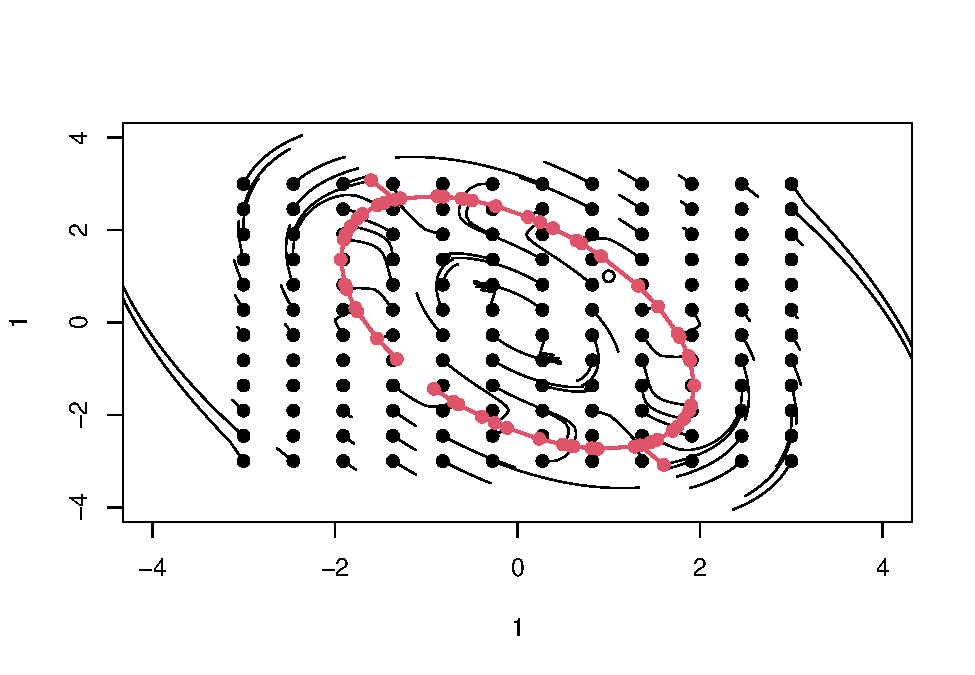
\includegraphics{Problemsetrmd_files/figure-latex/unnamed-chunk-13-1.pdf}

Now, we do the same thing for the f\_crois function.

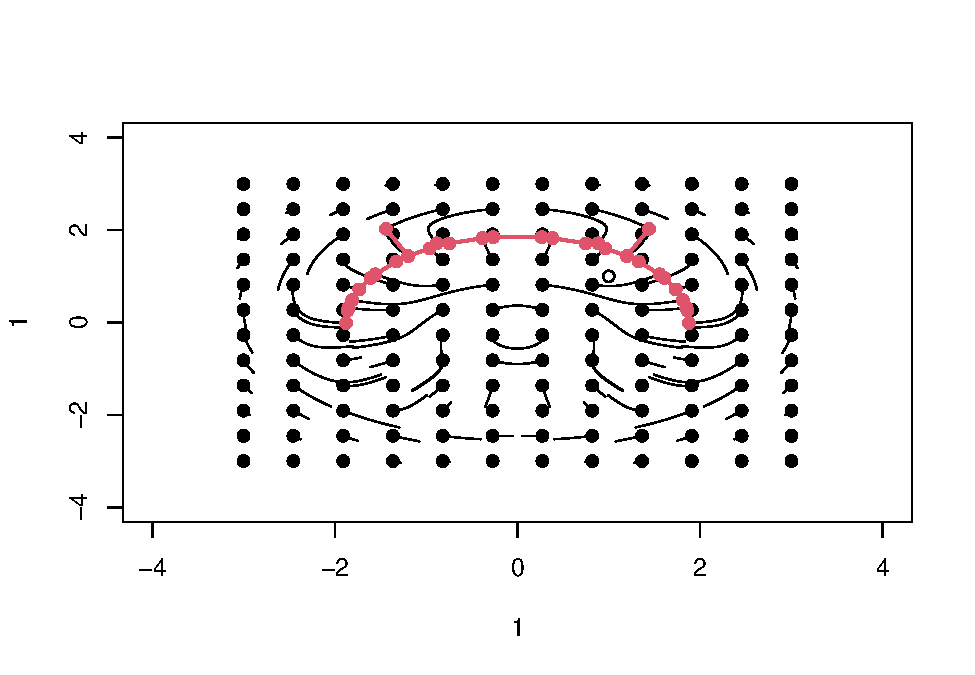
\includegraphics{Problemsetrmd_files/figure-latex/unnamed-chunk-16-1.pdf}

Now, same thing for f\_sin.

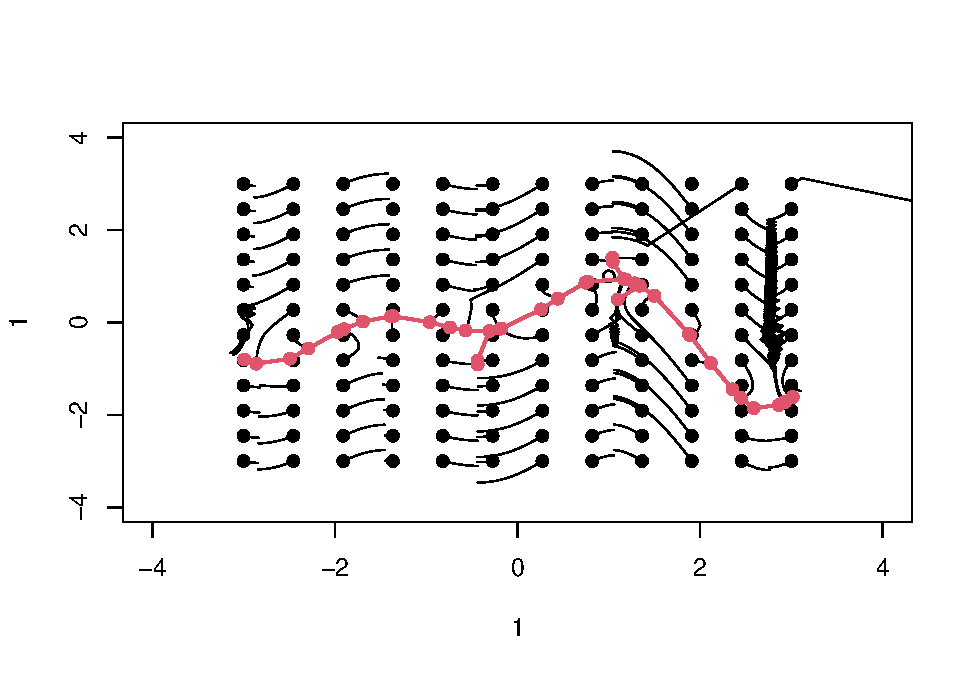
\includegraphics{Problemsetrmd_files/figure-latex/unnamed-chunk-19-1.pdf}

\end{document}
